% Generated by code/scripts/report_figures.py at 2026-11-06T09:28:43Z; do not edit.
% Inputs: artifacts/cluster/runs/bench16-20261105T092045Z-1523703
\begin{figure}[t]
\centering
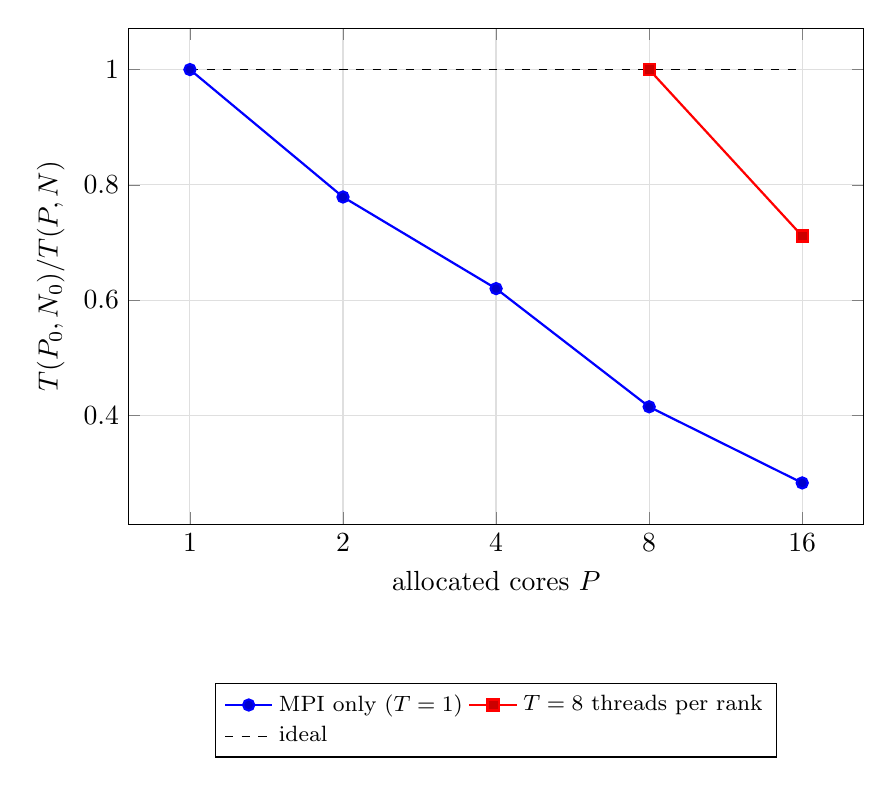
\begin{tikzpicture}
\begin{axis}[width=0.9\columnwidth, height=0.65\columnwidth, xlabel={allocated cores $P$}, ylabel={$T(P_0,N_0)/T(P,N)$}, xmode=log, log basis x=2, log ticks with fixed point, legend style={at={(0.5,-0.32)}, anchor=north, legend columns=2, font=\footnotesize}, legend cell align=left, grid=major, grid style={gray!25}]
\addplot+[mark=*, thick] coordinates {(1,1) (2,0.7789) (4,0.6199) (8,0.4148) (16,0.2827)};
\addlegendentry{MPI only ($T=1$)}
\addplot+[mark=square*, thick] coordinates {(8,1) (16,0.7111)};
\addlegendentry{$T=8$ threads per rank}
\addplot[black, dashed] coordinates {(1,1) (16,1)};
\addlegendentry{ideal}
\end{axis}
\end{tikzpicture}
\caption{Weak-scaling efficiency. $T=1$: $P_0=1$, $N_0=50000$, 50000 particles per core; $T=8$: $P_0=8$, $N_0=400000$, 50000 particles per core. Constant particles per core is not constant work per core. Vanda job 1523703: 16 cores of a shared Gold 6438N node, 3 interleaved repetitions.}
\label{fig:weak}
\end{figure}
